\section{Conclusion}
\begin{frame}
    \frametitle{Strengths}
    \begin{itemize}
        \item<1-> \textbf{Zero-shot learning}: CLIP can be used for a wide range of tasks without any fine-tuning
        \item<2-> \textbf{Human labor}: No manually labeled data is required
        \item<3-> \textbf{Performance}: CLIP matches or outperforms fine-tuned, specialized models in many tasks
        \item<5-> \textbf{Symmetry}: It's also possible classify a piece of text for a given set of images
    \end{itemize}
\end{frame}

\begin{frame}
    \frametitle{Weaknesses}
    \begin{itemize}
        \item<1-> \textbf{Performance}: For many tasks, CLIP is outperformed by specialized models
        \item<2-> \textbf{Prompting}: Sensitive to the input choices, may require prompt engineering to achieve good results
        \item<3-> \textbf{Bias} of the training data is encoded in the model
        \item<4-> \textbf{Dataset} is not publicly available, source is unclear
    \end{itemize}
\end{frame}

\begin{frame}
    \frametitle{Applications: StyleCLIP}
    Using CLIP to manipulate images with text prompts \footfullcite{patashnik2021styleclip}
    \includegraphics[width=\textwidth]{./images/teaser}
\end{frame}

\begin{frame}
    \frametitle{Applications: Client-side image search}
    Leverage symmetric nature of CLIP to sort/search for images using text prompts \footfullcite{clientsideimagesearch}
    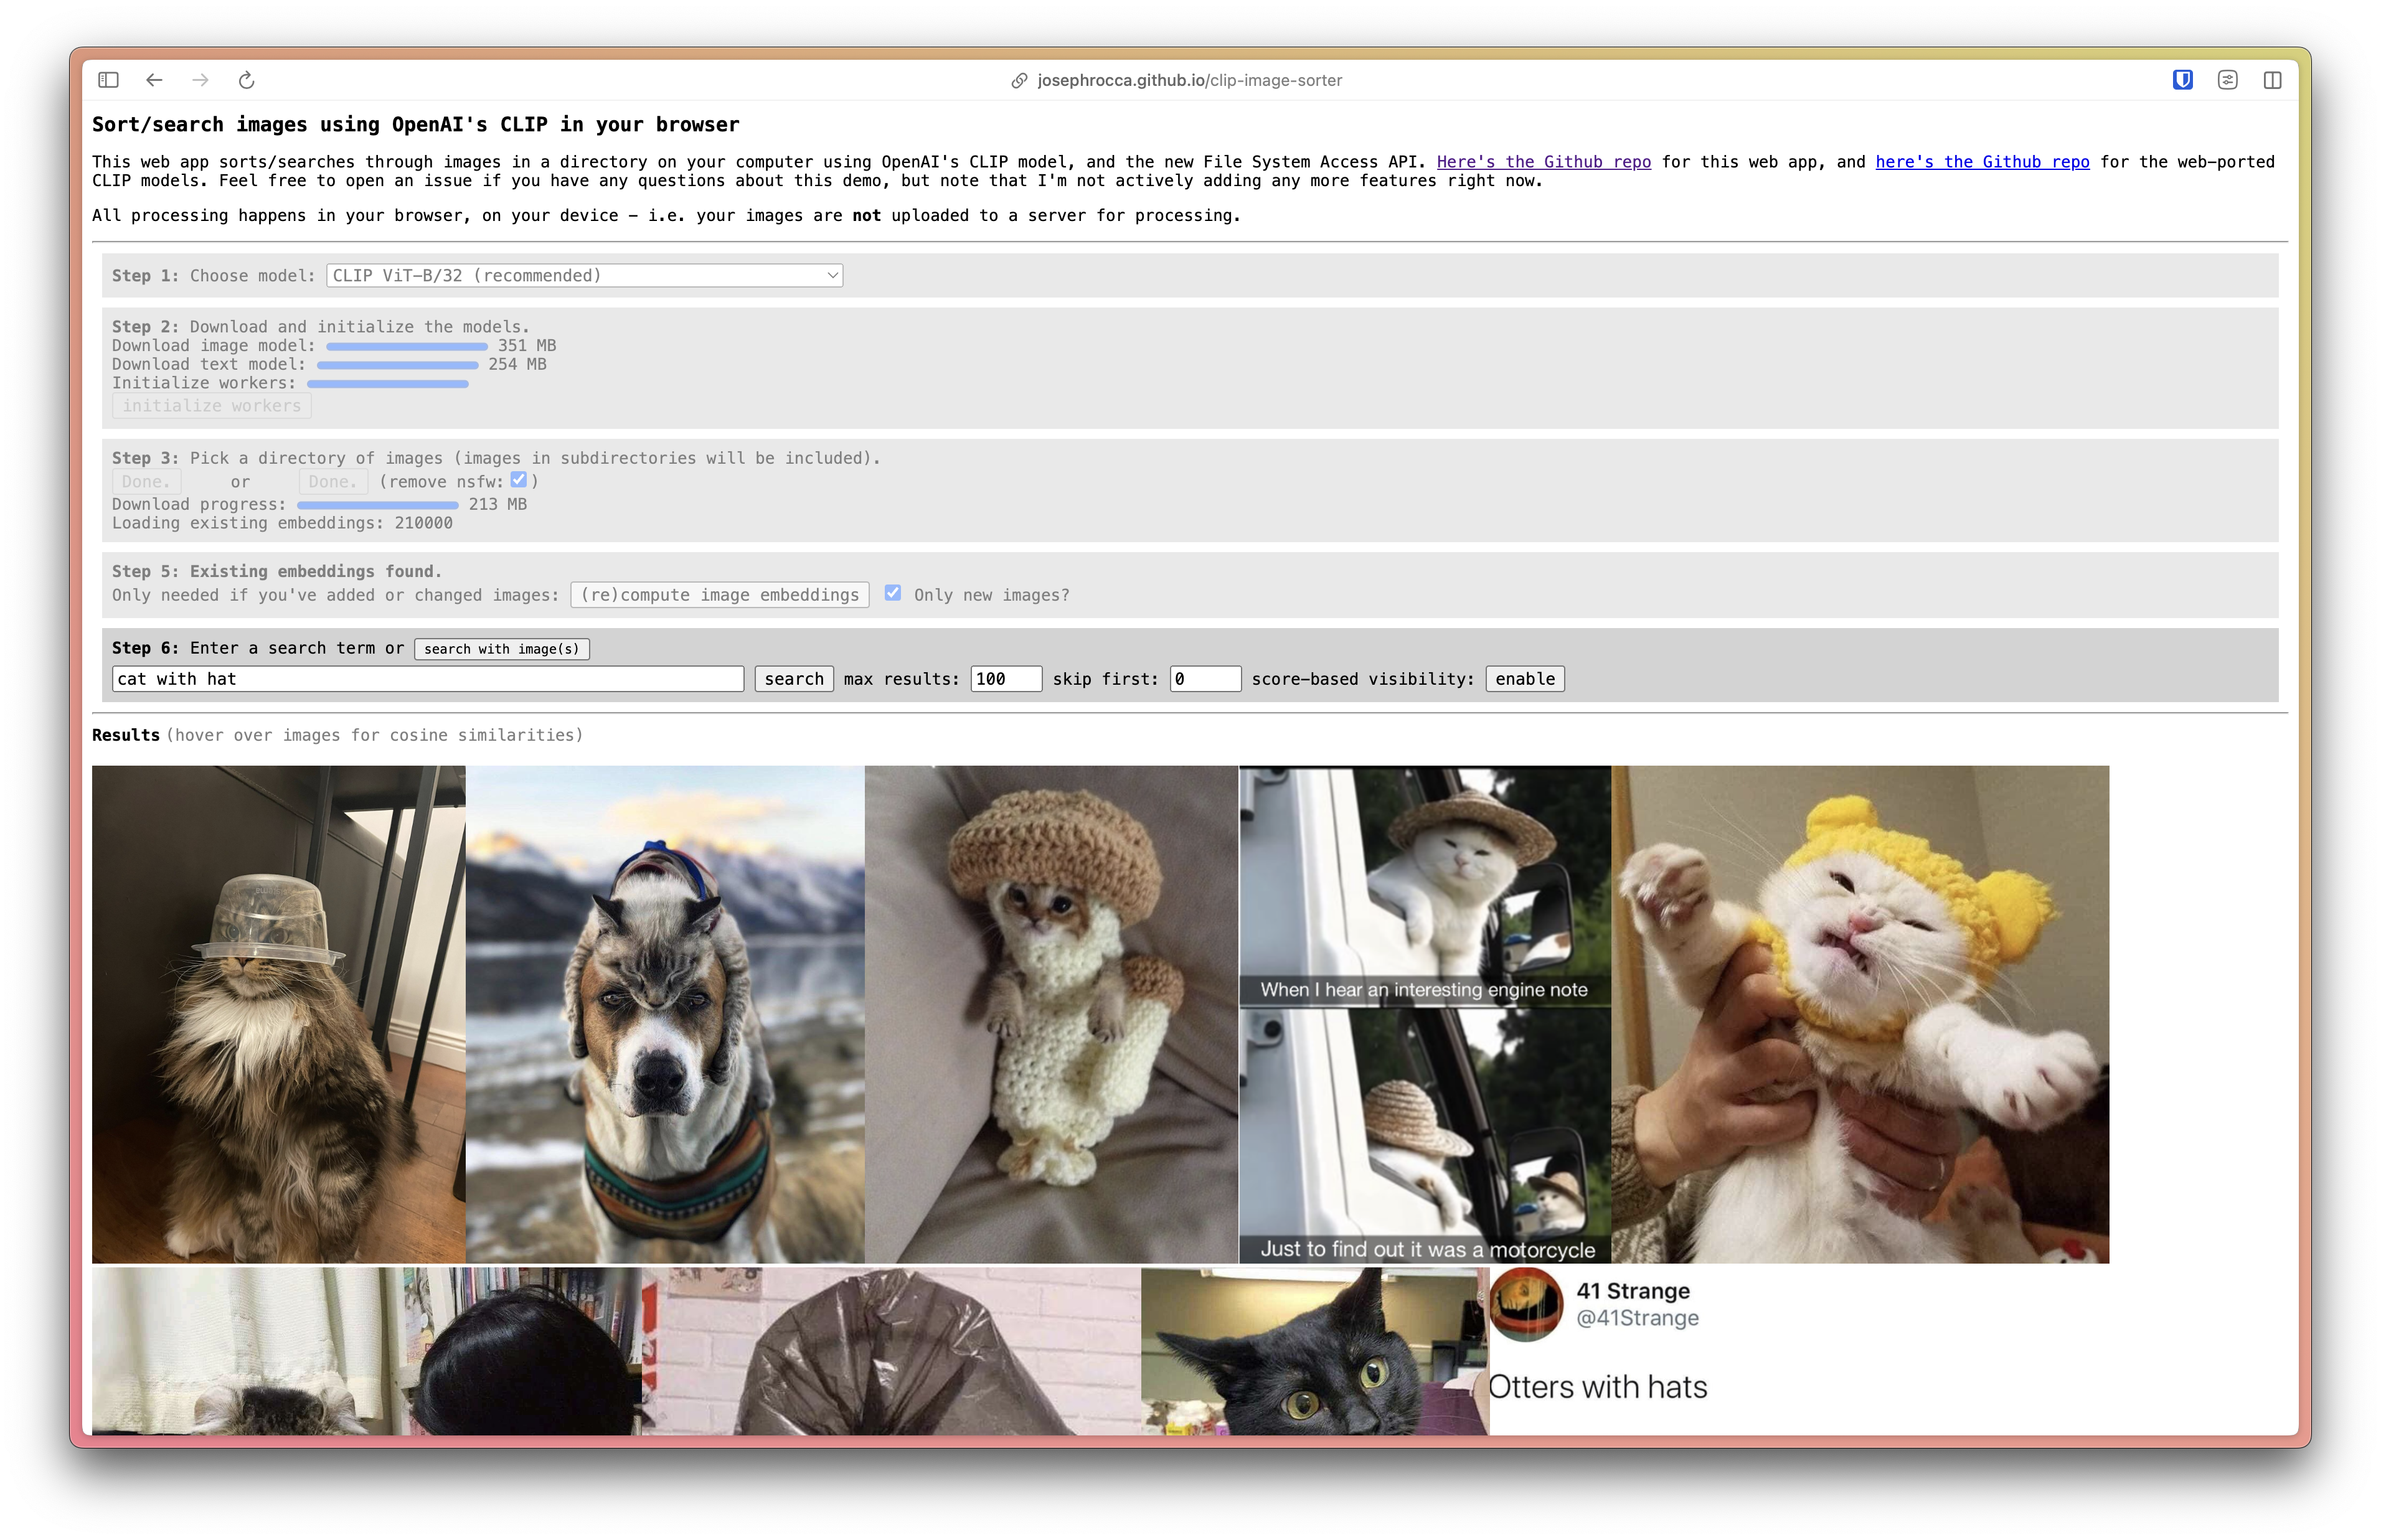
\includegraphics[width=8cm]{./images/image-search}
\end{frame}

\begin{frame}
    \frametitle{Applications: Image generation}
    Use CLIP to generate images from text prompts \footfullcite{ramesh2022hierarchicaltextconditionalimagegeneration}
    \includegraphics[width=12cm]{./images/unclip-figurehead}
\end{frame}
